\section{Dual Matroids}
The concept of \textit{duality} is an interesting feature of matroid theory. It helps to extend some of the constructions in our prototypical examples in representable and graphic matroids, such as the notion of orthogonality in vector spaces and the concept of a planar dual of a plane graph, to general matroids. In this section we will introduce the definitions and  properties of dual matroids.

%Before starting with the formal definitions, porperties and theorems is important that we state the most important concept of this chapter, that is, similar to the chapter name, the concept of a \textit{dual}, or more precisely, the \textit{dual of a matroid}.\\

% I DONT THING THE ABOVE PARAGRAPH ADDS ANY CONTENT

If we have a matroid $M$, with sets $(E,B)$, or in other words $M$ is a matroid on $E$ with $B$ as its collection of bases. Then its dual will refer to a different and new matroid, which we denote by $M*$. This new matroid has the property that it is "related" to the original matroid, so it has the same ground set $E$ of the original matroid $M$, but a different basis set, this new basis collection will be called $B*$, so this gives us that $M*$ will be defined by the following pair of sets $(E,B*)$. Where $B^*$ will a set such that is is the complement of the bases set $B$ in $M$, which implies that, the bases set of $M$ and $M^*$ will be always disjoint.

This can be seen more clearly in the following digram:
\begin{figure}[H]
    \centering
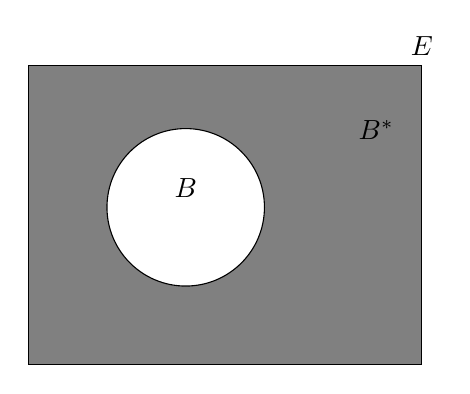
\begin{tikzpicture}
        \filldraw[fill=gray] (-2,-2) rectangle (3,1.8) node [text=black,above] {$E$} node at (19:3) [text= black, left = 2pt] {$B^*$};
        \scope % B
        \clip (0,0) circle (1);
        \fill[white] (0,0) circle (1.5);
        \endscope
        \draw (0,0) circle (1) node [text=black,above] {$B$};
\end{tikzpicture}
\caption{Venn diagram showing, B the basis set of $M$, and $B^*$ the basis set of $M^*$}%
\label{graphic}%
\end{figure}

We also have the depiction from previous sections, but know we will also the one that will correspond to the dual on this specific case. To the \textbf{left} we have the depiction corresponding to the \textbf{original matroid}, and to the \textbf{rigth} we have the one corresponding to its \textbf{dual matroid}. 
Notice how the ground set will be composed of 4 components $E=\{1,2,3,4\}$, and in the original matroid has bases $12$ and $23$, in red. So, its dual has bases $34$ and $14$, respectively, also in red but in the rigth-side diagram. This is because, the complement of the elements $12$ is $34$, and the complement of $23$ is $14$.


\begin{tikzpicture}[H]
\centering
\matrix (a) [matrix of math nodes, column sep=0.3cm, row sep=0.6cm,]{
 & & &\textcolor{cyan}{
1234} & & & &\\
 \textcolor{cyan}{
123}& &\textcolor{cyan}{
124} & &\textcolor{cyan}{
134} &  & \textcolor{cyan}{
234}  \\
\textcolor{red}{12} & \textcolor{blue}{13} & \textcolor{cyan}{14} & & \textcolor{red}{23} & \textcolor{cyan}{
24} & \textcolor{cyan}{
34} \\
\textcolor{orange}{1}& &\textcolor{orange}{2} & & \textcolor{orange}{3}& & \textcolor{blue}{4} \\
& & & \textcolor{orange}{\emptyset} &  & & \\
&&&&&& \\};

\foreach \i/\j in {1-4/2-1, 1-4/2-3, 1-4/2-5, 1-4/2-7, 2-1/3-1, 2-1/3-2, 2-1/3-5, 2-3/3-1, 2-3/3-3, 2-3/3-6, 2-5/3-2, 2-5/3-3, 2-5/3-7, 2-7/3-5, 2-7/3-6, 2-7/3-7, 3-1/4-1, 3-1/4-3, 3-2/4-1, 3-2/4-5, 3-3/4-1, 3-3/4-7, 3-5/4-3, 3-5/4-5, 3-6/4-3, 3-6/4-7, 3-7/4-7, 3-7/4-5, 4-1/5-4, 4-3/5-4, 4-5/5-4, 4-7/5-4}
\draw[double, line width = 0.005mm, color = brown] (a-\i) -- (a-\j);

\end{tikzpicture}
\begin{tikzpicture}[H]
\centering
\matrix (a) [matrix of math nodes, column sep=0.3cm, row sep=0.6cm,]{
 & & &\textcolor{cyan}{
1234} & & & &\\
 \textcolor{cyan}{
123}& &\textcolor{cyan}{
124} & &\textcolor{cyan}{
134} &  & \textcolor{cyan}{
234}  \\
\textcolor{cyan}{12} & \textcolor{blue}{13} & \textcolor{red}{14} & & \textcolor{cyan}{23} & \textcolor{cyan}{
24} & \textcolor{red}{
34} \\
\textcolor{orange}{1}& &\textcolor{blue}{2} & & \textcolor{orange}{3}& & \textcolor{orange}{4} \\
& & & \textcolor{orange}{\emptyset} &  & & \\
&&&&&& \\};

\foreach \i/\j in {1-4/2-1, 1-4/2-3, 1-4/2-5, 1-4/2-7, 2-1/3-1, 2-1/3-2, 2-1/3-5, 2-3/3-1, 2-3/3-3, 2-3/3-6, 2-5/3-2, 2-5/3-3, 2-5/3-7, 2-7/3-5, 2-7/3-6, 2-7/3-7, 3-1/4-1, 3-1/4-3, 3-2/4-1, 3-2/4-5, 3-3/4-1, 3-3/4-7, 3-5/4-3, 3-5/4-5, 3-6/4-3, 3-6/4-7, 3-7/4-7, 3-7/4-5, 4-1/5-4, 4-3/5-4, 4-5/5-4, 4-7/5-4}
\draw[double, line width = 0.005mm, color = brown] (a-\i) -- (a-\j);
\end{tikzpicture}

\begin{center}
\begin{tikzpicture}[H]
\centering
\node[draw] at (0, -2.5){\small \textcolor{orange}{Independent set}, \textcolor{red}{Basis}, \textcolor{blue}{Circuit}, \textcolor{cyan}{Dependent set}}
\end{tikzpicture}
\end{center}




We know that the basis set of a matroid is obtained from its set of independet sets $I$.
Using this diagrams we highligth an idea that will be useful later in this chapter.
This is, that the basis set of a matroid is given by a subset of $E$, the remaing elements in $E$ that are not in de basis if added to the basis will be linearly dependent, but also we can take any remaining element of $E$ and exchange it with an element in the basis and we will have another basis for $E$. With this intuition in mind, we can continue with a theorem.


To formalize the definition of $B^*$ we have the following:
\begin{theorem}
    Let $M$ be a matroid given by $(E,B)$, and B*$(M)$ be $\{E(M) - B:B\in B(M)\}$. Then B*$(M)$ is the set of bases of a matroid on $E(M)$
\end{theorem}

Or in other words, B* is the set of all the complement independent bases of $B$. Then we can give the following definition.

\begin{defn}
    Let M be a matroid with the pair (E,B), given B* as defined above, the new matroid M*=(E,B*) is the dual of M.
\end{defn}

In the theorem we say that B*$(M)$ is the set of bases of a matroid on $E(M)$, but this is not be trivially clear, so we need to prove it.

However to prove it we will mahe use of the following result, that comes from our properties of the basis set B of our matroid M in Section 2.2

Lemma. The set $B$ of bases of a matroid M has the following property:
$(B2)^*$ If $B_1$ and $B_2$ are in B and $x \in B_2 - B_1$,then there is exist and element $y$ of $B_1 - B_2$ such that $(B_1 - y) \cup x \in B$

\textit{For comparison this was the original (B2): \\
$(B2)$ If $B_1,B_2\in\mathcal{B}$ and $x\in B_1 - B_2$, then there exists a $y\in B_2 - B_1$ such that $(B_1 - x)\cup y \in\mathcal{B}$.}\\

First we will prove $(B2)^*$:
\begin{proof}
  We note that $B_1$ is by definition a base, this means that if we add a new element in the ground set to it, it will become a minimal dependet set, in other words $B_1 \cup x$ contains a unique circuit $C_1 \in C$. Since we have $C_1$ a dependent set and $B_2$ another base, and thus independet, then $C_1 - B_2$ will be non-empty, so there exists and element $y$ such that $y \in C_1 - B_2$, but as $C_1$ is the circuit created from $B_1 \cup x$, then $y \in (B_1 \cup x) - B_2$, but as $x \neq y$, then $y \in B_1 - B_2$. Now, lets take $B_1 - y$, this will not be a basis, but it will be an independent set, if now we take $(B_1 - y)\cup x$, this will clearly not contain the circuit $C_1$, since this was the unique circuit generated from $B_1 \cup x$, so the set $(B_1 - y)\cup x$ must be independent. Finally, we observe that $(B_1 - y)\cup x$ implies that we add and elemnts to the set and we take out one element to the set, so the cardinality will remain equal, that is: $|(B_1 - y)\cup x|=|B_1|$.
As we have that $(B_1 - y)\cup x$ is and independent set and has the same cardinality as the the base $B_1$, then by definition $(B_1 - y)\cup x$ is also a base.  
\end{proof}

Now, we prove that $B^*(M)$ is the set of a base of a matroid on $E(M)$
\begin{proof}
    As $B(M)$ is non-empty, $B^*(M)$ is non-empty, hence, the property $(B_1)$ holds for $B^*(M)$. 
    Now, consider two members of $B^*(M)$, $B^*_1$ and $B^*_2$, not equal such that there exists an element $x \in (B^*_1 - B^*_2)$. Let, $B_1 = E - B^*_1$ and $B_2 = E - B^*_2$. We can see that $B^*_1 - B^*_2 = B_2 - B_1$, thus $x \in B_2 - B_1$. By $(B2)^*$, there exists and element $y \in  B_1 - B_2$ such that $(B_1 - y)\cup x$ is a base of $M$, but observe that $B_1 - B_2 = B^*_2 - B^*_1$, hence this is the same as saying that there exists and element $y \in  B^*_2 - B^*_1$ such that $(B_1 - y)\cup x$ is a base of $M$. Hence, by definition of dual, $E-((B_1 - y)\cup x) \in B^*(M)$. But, $E-((B_1 - y)\cup x) = ((E-B_1)-x)\cup y) = (B_1^* - x)\cup y$, which is in the family $B^*$. Thus, $B^*(M)$ satisfes $(B2)$. As $B^*(M)$ satisfies properties $(B1)$ and $(B2)$, this is indeed the set of bases of a matroid on $E$.
\end{proof}

The matroid M*, is the dual of M. Note that by the way is defined, and thanks to the proof above we see that $B(M^*)=B^*(M)$, moreover, due the nature that the definition of dual has, this is, that is the complement of the basis set, we have that
\begin{itemize}
    \item \textit{The dual of the dual of a matroid M is the matroid M itself, $i.e., (M^*)^* = M$}
\end{itemize}
This is because if we take the complement $B^*$ of the basis set $B$, and then we take this complement $B^*$ and take its complement once again, we will return to the original set $B$, or in other words: If $E-(E - B) = B$.\\

As an example, let $U_{k,n}$, be a k-uniform matroid. We know that its bases will be all the k-element subsets of $E(U_{k,n})$, we know that this matroid is defined over a set of $n$ elements, and its basis has exactly $k$ elements, hence the bases of $U_{k,n}$* are be all $(n-k)-element$ subsets of the ground set, as this will be the complement of the basis set of $U_{k,n}$. This is equal to saying that the dual of the matroid $U_{k,n}$ is given by $U_{k,n}$* $= U_{n-k,n}$\\


Now that we have introduced duals is useful to give some additional notation. That is, given a matroid $M$ with a dual $M^*$, the \textit{bases} of the matroid $M^*$ are called \textit{cobases} of $M$. Similarly, the \textit{independent sets} of $M^*$ are called \textit{coindependent sets} of $M$, the circuits of $M^*$ are called \textit{cocircuits} of $M$, \textit{hyperplanes} are called \textit{cohyperplanes}, and the \textit{spanning sets} are called \textit{cospanning sets} of $M$ and so on.\\

This leads us to some elemenary relationships between these sets. 

$Proposition:$ Let M be a matroid in a set E and suppose $X \subseteq E$. Then,
    \begin{enumerate}
        \item $X$ is independent if and only if $E-X$ is cospanning.

        \item $X$ is spanning if and only if $E-X$ is coindependent.

        \item $X$ is a hyperplane if and only if $E-X$ is a cocircuit

        \item $X$ is a circuit if and only if $E-X$ is a cohyperplane.
    \end{enumerate}

\begin{proof}
    All of the proofs follow directly from the definitions. [We will prove a) and b)]

    a) Suppose $X$ is independent. This means there exists a basis $B \in \mathcal{B}(M)$ so that $X \subset B$. Because $X \subset B \subset E$ and the operation of taking complements is "inclusion reversing" we have $E-B \subset E - X$. Verifying directly, if $x \in E - B$ this means $x \in E$ and $x \notin B$. Because $X \subset B$ this implies that $x \in E$ and $x \notin X$ so by definition $x \in E - X$ and the conclusion follows. Because $E - B$ is a cobasis and $E - X$ is a set containing a cobasis, then it is a cospanning by definion.

    Similarly if $E - X$ is cospanning then it contains a cobasis which is by definition of the form $E - B$ for some $B \in \mathcal{B}(M)$. By the analagous reasoning as for the forward direction $E - B \subset E - X$ implies $X \subset B$. That is because if $x \in X$ then $x \notin E - X$ and $x \notin X - B$. This means $x \in B$ concluding $X \in B$. Since $B$ is an independent set then $X$ is independent set as well, we are done.

    b) Same as a). A set $X\subset E$ being spanning implies it contains a $B \in \mathcal{B}(M)$. So  $B \susbet X$ which implies $E - X \subset E - B$. Because $E - B$ is cobasis by definition, any of its subsets are coindependent. 

    If $E - X$ is coindependent, it is contained in a cobasis, so by definition there exists a $B \in \mathcal{B}$ so that $E - X \subset E - B$. As before this implies that $B \subset X$ and $X$ is spanning.

    c)  If $X$ is a hyperplane, then $X$ is not spanning but for all $y \in E - X$ we have $X \cup y$ is spanning, which means there is for every such $y$ a basis $B_y \in \mathcal{B}$ so that $B_y \subset X \cup y $. By b) we know that $X$ is not spanning implies $E - X$ is not coindependent. But for any $z \in E - X$ we have $(E-X)-z = E - (X \cup z)$ is coindependent because $X \cup z$ is spanning. So $E - X$ is a cocircuit by definition.

    Conversly, if $E - X$ is a cocirucuit, then $E-X$ is not coindependent but for all $x \in E - X$ we have $(E - X) - x$ = $E - (X \cup x)$ is coindependent. By b) this means that $X$ is not spanning but for all $x \in E-X$, we have $X \cup x$ is spanning, so $X$ is a hyperplane.

    d) Same as things before.
\end{proof}\\

Similar to the case with the bases and cobases, the rank function of the dual matroid is usually denoted by $r^*$, and is normally referred as the $corank$ $function$ of $M$. Using the definition of bases of the dual matroid, this is, that is build with the complement bases of the set of the orginal matroid, as well as the fact that matroid and its dual are both on the same ground set, we have the following:

\begin{itemize}
    \item $r(M) + r$*$(M) = |E(M)|=|E(M^*)|$
\end{itemize}

And in fact, we can generalize this to obtain an explicit formula for the for the corank function of the matroid. 

For all subsets X of the ground set E of a Matroid M,
\begin{itemize}
    \item $r^*(X)=r(E-X)+|X|-r(M)$
\end{itemize}

\begin{proof}
    Let $I^*$ be a independet subset of $X$ in $M^*$, such that it is not a subset of some other set in $X$, this is $r^*(X)=|I^*|$. Similarly, let $I$ be a independent subset of $E-X$ in $M$, such that it is not a subset of some other set in $E-X$, this is $r(E-X)=|I|$. And let $B$ be an independent subset of $E-I^*$, such that it is not a subset of some other set in $E-I^*$ and contains $I$. Since, this are independent subsets that are not subsets of any other element in their respective sets, then we have $r(B)=r(E-I^*)$ and $r(E-I^*)=r(M)$, and hence $B$ is a base of M.
    Now, let $B^*=E-B$, since $B$ is a base of $M$, by definition $B$ is a base of $M^*$. We can onserve that $I^*\subseteq B^*$ and  $B^*\cap X=I^*$. Similarly, $I\subseteq B$ and  $B\cap (E-X)=I$. In particular we see that, $|B\cap X|=|B|-|I|$, thus
    $|X|=|X\cap B|+|X\cap B^*|=|B|-|I|+|I^*|=r(M)-r(E-X)+r^*(X)$
\end{proof}


%Subsection
Now we will talk about duals of representble matroids.
Let A be an $m \times n$ matrix over the field $F$, and let M be vector matroid $M[A]$ of $A$. Then we have that the groud set of $M$ is the set $E$ of column labels of $A$. Note that, in general, $M[A]$ does note uniquely determine $A$. Furthermore, M remains unchanged if we perform any of the following operarations on $A$, which include the \textit{elementary row operations} seen in the linear algebra courses.
\begin{enumerate}
    \item Interchange two rows.
    \item Multiply a row by a non-zero member of $\mathbb{F}$.
    \item Replace a row by the sumof that row with another row.
    \item Adjoin or remove a zero row.
    \item Interchanging two columns (the labels moving with the columns).
    \item Multiply a column by a non-zero member of $\mathbb{F}$.
\end{enumerate}

The reason for this is because when constructiong the matroid $M$ form a matrix $A$, we only care about the independence (or dependence) that each column vector in the matrix has with one another. So, as long as the independence and dependece between this is keep the same, the values inside the columns are not relevant.

Assume that the matrix A is non-zero. It is known that by using the operations previusly mentioned A can be reduced to be of the form $[I_r|D]$, where $I_r$ is the $r \times r$ identity matrix and $D$ is some $r \times (n-r)$ matrix over $F$. We can clearly see that $r(M)=r$ (the dimension fo the identity matrix). 

Suppose that the columns of $[I_r|D]$ are labelled, in order, in the following form, $e_1, e_2,...,e_n$. This will be the ground set $E=\{e_1, e_2,...,e_n\}$. Then, we see that $\{e_1, e_2,...,e_r\}$ is a basis $B$ of $M$, once agina due to the dimesion of the identity matrix. We also label both, the rows and colums of $D$, in the following form, for the rows from top to bottom, $e_1, e_2,...,e_r$ and for the columns,  $e_{r+1}, e_{r+2},...,e_n$. This way to represent $M[A]$ can be seen more clearly in the following figure. We will refer to both $[I_r|D]$ and $D$ as the \textit{standard representative matrices} for $M$, \textit{with respect to $\{e_1, e_2,...,e_r\}$}. Similarly, we use \textit{reduced standard representative matrix} if we want to refer only to $D$.

\begin{figure}[H]
    \centering
    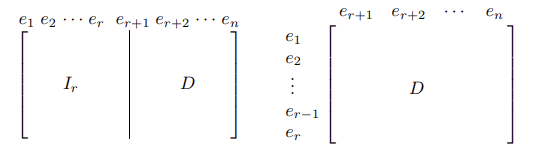
\includegraphics{SRF.png}
    \caption{Standard representative matrices for M. [3]}
    \label{fig:enter-label}
\end{figure}
Note that, in the figure, in $[I_r|D]$ only the columns are labelled, but in $D$, both the rows and columns ae labeled.

We can now use this construction to determine the dual of a vector matroid using the following theorem.

\begin{theorem}
    Let M be the vector matroid of the matrix $[I_r|D]$ where the columns of this matrix are labelled, in order, $e_1, e_2,...,e_n$ and $1\leq r< n$. Then $M^*$ is the vector matroid of $[-D^T|I_{n-r}]$ where its columns are also labelled $e_1, e_2,...,e_n$ in that order.
\end{theorem}

\begin{proof}
    We assume that $[I_r|D]$ is as in the contruction of the theorem above. Then $[-D^T|I_{n-r}]$ is as follows


    Let $B$ be a basis of $M$. We need to show that $E-B$ is a basis of the vector matroid of $[-D^T|I_{n-r}]$. We can rearrege the columns of $[-D^T|I_{n-r}]$, such that $B=\{e_1,\dots,e_s, e_{r+1}, \dots , e_{r+(r-s)}$, for some $s \leq r$. This is possible becasue we know that it does not affect the corresponding matroid, so the only change it bring to rearrange rows and columns of $[I_r|D]$ is the re-arrenge of columns and rows of $[-D^T|I_{n-r}]$. 
    
    Using this we can partition $[I_r|D]$ in the following form
    \begin{figure}[H]
    $$\begin{bmatrix}
    I_s & 0 & D_{11} & D_{12\\
    0 & I_{r-s} & D_21 & D_22\\
    \end{bmatrix}
    % 
    \rightarrow
    \begin{bmatrix}
    -D_{11}^T & -D_{21}^T & I_{r-s} & 0\\
    -D_{12}^T & -D_{22}^T & 0 & I_{n-(2r-s)}\\
    \end{bmatrix}$$
    \end{figure}
    First, lets analyse the partition of $[I_r|D]$.
    Here me made the partition such that the first component $I_s$ has columns from $(e_1 \dots e_s)$. $I_{r-s}$ has columns from $(e_{s+1} \dots e_r)$, $D_11$ and $D_21$ have from $(e_{r+1} \dots e_{2r-s})$, and finally $D_12$ and $D_22$ have from $(e_{(2r-s)+1} \dots e_n)$.
    
    We have that $B$ is a base, this means that it must have the same size as $I_r$. Due to the way the matrix $[I_r|D]$ is partitioned, that is, if the we take the components in the partirion that contain the columns of the basis we have the following matrix:
    \begin{figure}[H]
        \centering
        $$\begin{bmatrix}
        I_s & D_{11}\\
        0 & D_{21}\\
        \end{bmatrix}$$
    \end{figure}
    As this matrix has the components that contain all the elements in the basis implies that it must have $rank = r$ (the rank of $[I_r|D]$), but here $I_s$ has $rank = s$, as it is the identity matrix. Hence, the the rank of $D_11$ is $r-s$, which also corresponds to the rank of $D_21^T$.
    
    If we now observe the partition of $[-D^T|I_{n-r}]$, this will gave the same partition lengths in each component as the ones mentioned for $[I_r|D]$ above. 
    
    in the rigth side, we notice that following a similar reasoning this will have a rank of $n-(2r-s)$    
\end{proof}

By convention the form $[−D^T |I_{n−r}]$ instead of $[D^T |I_{n−r}]$. However it is important to remark that this does not bring any problem, because, as we previusly stated, the use of \textit{elementary row operations} does not affect the matroid of a matrix. 

From the previous theorem a remarkable result follows almost directly. 
\begin{itemize}
    \item  \textbf{Corollary 1. :} If a matroid \textit{M} is \textit{representable} over a field $\mathbb{F}$, then \textit{M*} is also representable over the same field $\mathbb{F}$.
\end{itemize}


$Example:$ Consider the vector matroid $M$ with the following representation over $R$
        \begin{figure}[H]
            $$A = \begin{bmatrix}
                1 & 0 & 0 & 1 & 0 & 1 \\
                0 & 1 & 0 & 1 & -1 & 0 \\
                0 & 0 & 1 & 0 & 1 & 1 \\
            \end{bmatrix}$$
        \end{figure}
        
The by the theorem the corresponding dual matroid $M^*$ is the vector matroid represented by 
        \begin{figure}[H]
            $$A^* = \begin{bmatrix}
                -1 & -1 & 0 & 1 & 0 & 0 \\
                0 & 1 & -1 & 0 & 1 & 0 \\
                -1 & 0 & -1 & 0 & 0 & 1 \\
            \end{bmatrix}$$
        \end{figure}
As and interesting note, this vector matroid $A$ is associated to the graph $K_4$ 
       \begin{figure}[H]
        \centering
            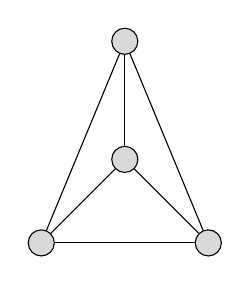
\begin{tikzpicture}[
                node distance = 15mm and 15mm,
                V/.style = {circle, draw, fill=gray!30},
                every edge quotes/.style = {auto, font=\footnotesize, sloped}
                    ]
                \begin{scope}[nodes=V]
                \node (1) {}; 
                \node (2) [below of=1] {}; 
                \node (3) [below left of=2] {}; 
                \node (4) [below right of=2] {}; 
                \end{scope}
                \draw (1) to (2); 
                \draw (1) to (3);
                \draw (1) to (4); 
                \draw (2) to (3);
                \draw (2) to (4); 
                \draw (3) to (4);
            \end{tikzpicture}
            \caption{$K_4$, the complete graph on 4 vertices}
            \label{fig:enter-label}
        \end{figure}

Aditionally, from this we can also verify the $rank$ and $corank$ propositions established before. This is, we can clearly observe that $A$ has a ground set $E=\{e_1, e_2, \dots , e_6\}$ with 6 elements, where each $e_i; i =1,2, \dots,6$ represents a column, hence $|E|=6$. We also see that $A$ has rank $r(A)=3$, which can be easily verified by observing the first 3 columns that correspond to the identity matrix in the construction of the form $[I_r|D]$. Similarly, if we observe the dual we notice that also $r(A^*)=3$. \\So, $r(A)+r(A^*)= 3 + 3 = 6 = |E|$\\


%

We have seen many concepts related to dual matroids, including some representations for vector matroids, however we have not gone that much into detail with graphic matroids. So, the reader could still be wondering, \textit{"Is it possible to have a graphic matroid whose dual is not grahic?"}

To answer that we have the following theorem

\begin{theorem}
    \item  The dual of a graphic matroid is itself graphic if and only if the underlying graph is planar.
\end{theorem}

\begin{proof}
    TODO
    Hello
\end{proof}



$Example:$ Let us consider the bipartite graph $K_{3,3}$.
\begin{figure}[H]
\centering
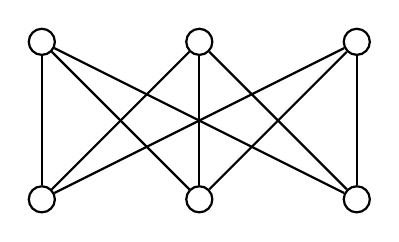
\begin{tikzpicture}[node distance={20mm}, thick, main/.style = {draw, circle}] 
    \node[main] (1) {}; 
    \node[main] (2) [below of=1] {}; 
    \node[main] (3) [right of=1] {}; 
    \node[main] (4) [below of=3] {}; 
    \node[main] (5) [right of=3] {}; 
    \node[main] (6) [below of=5] {}; 
    \draw (1) to (2); 
    \draw (1) to (4);
    \draw (1) to (6); 
    \draw (3) to (2);
    \draw (3) to (4); 
    \draw (3) to (6);
    \draw (5) to (2); 
    \draw (5) to (4);
    \draw (5) to (6);
    \end{tikzpicture}
    \caption{The bipartite graph $K_{3,3}$}
    \label{fig:enter-label}
\end{figure}

We can see it has 9 edges, so the ground set is $E=\{1,2,3, \dots, 9\} $.

\begin{figure}[H]
The matrix associated to the matroid $M(K_{3,3})$ is the following:
$$J = \begin{bmatrix}
    1 & 0 & 0 & 0 & 0 & 1 & 0 & 0 & 1\\
    0 & 1 & 0 & 0 & 0 & 1 & 1 & 0 & 1\\
    0 & 0 & 1 & 0 & 0 & 1 & 1 & 1 & 1\\
    0 & 0 & 0 & 1 & 0 & 0 & 1 & 1 & 1\\
    0 & 0 & 0 & 0 & 1 & 0 & 0 & 1 & 1\\
\end{bmatrix}$$
\end{figure}

This is because if we label the columns of $J$ as $E = \{e_1,\dots, e_9\}$ and define a matroid $M(J)$ on $E$, it is easy to see that we associate each column of $J$ to the correspondingly labeled edge in $K_{3,3}$, so that they generate the same matroid. Moreover, this means that we can take a basis for the column space of $J$, such as, $B = \{e_1, e_2, e_3, e_4, e_5\}$, such that it corresponds to a spanning tree $T$ of $K_{3,3}$ (See Figure 8.). In other words, this means that adding any other column to $J$ gives a linear dependency, more precisely a circuit in $M(J)$, and adding any edge to $T$ generates a cycle.
\begin{figure}[H]
    \centering
    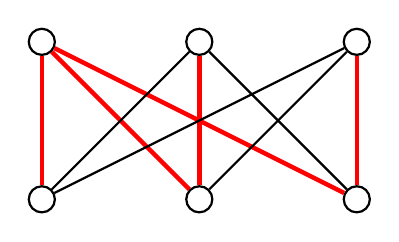
\begin{tikzpicture}[node distance={20mm}, thick, main/.style = {draw, circle}] 
        \node[main] (1) {}; 
        \node[main] (2) [below of=1] {}; 
        \node[main] (3) [right of=1] {}; 
        \node[main] (4) [below of=3] {}; 
        \node[main] (5) [right of=3] {}; 
        \node[main] (6) [below of=5] {}; 
        \draw [ultra thick,red] (1) to (2); 
        \draw [ultra thick,red] (1) to (4);
        \draw [ultra thick,red] (1) to (6); 
        \draw (3) to (2);
        \draw [ultra thick,red] (3) to (4); 
        \draw (3) to (6);
        \draw (5) to (2); 
        \draw (5) to (4);
        \draw [ultra thick,red] (5) to (6);
    \end{tikzpicture}
    \caption{Graph $K_{3,3}$, showing in red an example of edges that form a spanning tree, that can be associated accordingly to the basis of $J$.}
    \label{fig:enter-label}
\end{figure}

Now that we have show that $K_{3,3}$ has an associated matrix, which produces the same Matroid, we can use the Theorem 12. to obtain the corresponding dual. 
So we get, 
\begin{figure}[H]
  $$J^*=\begin{bmatrix} 
1 & 1 & 1 & 0 & 0 & 1 & 0 & 0 & 0\\
0 & 1 & 1 & 1 & 0 & 0 & 1 & 0 & 0\\
0 & 0 & 1 & 1 & 1 & 0 & 0 & 1 & 0\\
1 & 1 & 1 & 1 & 1 & 0 & 0 & 0 & 1\\
\end{bmatrix}$$
\end{figure}

As a sanity check we can see that;
$r(J) = 5$;  $r^*(J)=4$, and $|E(M)|=9$
Hence, we see that $r(M) + r^*(M) = |E(M)|$ holds.
According to the \textbf{Corollary 1.}, \textit{If a matroid \textit{M} is \textit{representable} over a field $\mathbb{F}$, then \textit{M*} is also representable over $\mathbb{F}$} , here we see that, both matroids are vector matroids over the field $\mathbb{F}_2$. 
Finally, in this example we can observe that $K_{3,3}$ is not a planar graph, this implies that, although $M(K_{3,3})$ is a graphic matroid, its dual, $M^*(K_{3,3})$ is not graphic.

